%!TEX root = notes.tex

\chapter{Unconstrained Optimization via Calculus}


The image of a continuous functions enjoys nice properties, which are key to the pursue of extrema.  Let's start with two basic Theorems.

\begin{theorem}[Bounded Value Theorem]\label{theorem:BVT}
The image $f(K)$ of a continuous real-valued function $f \colon \field{R}^d \to \field{R}$ on a compact set $K$ is bounded: there exists $M>0$ so that $\abs{ f(\x) } \leq M$ for all $\x \in K$.
\end{theorem}

\begin{theorem}[Extreme Value Theorem]\label{theorem:EVT}
A continuous real-valued function $f \colon K \to \field{R}$ on a compact set $K \subset \field{R}^d$ takes on minimal and maximal values on $K$.
\end{theorem}

Theorem \ref{theorem:EVT} guarantees the existence of global extrema for continuous real-valued functions over compact subsets.  % What if we do not have compactness?



% It is the behavior of the interaction of the rest of the graph with this hyperplane what will give us clues to the nature of possible extrema.

% \begin{figure}[ht!]
% \begin{tabular}{cc}
% %  &
% % 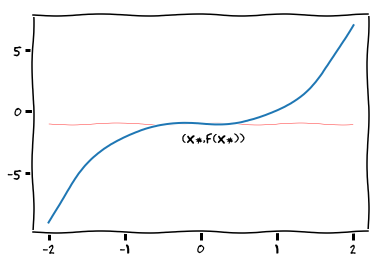
\includegraphics[width=0.45\linewidth]{x3.png}
% \begin{tikzpicture}
% \draw [white] (-2,-2) rectangle (2,2);
% \draw (0,0) node{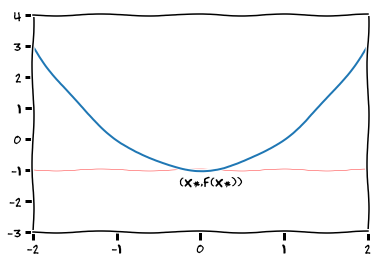
\includegraphics[width=0.5\linewidth]{x2.png}};
% % \draw [smooth, samples=100, domain=-1.732:1.732, blue, ultra thick, variable=\t] plot({\t}, {\t*\t-1});
% % \draw[thick] (-2,-1) -- (2,-1);
% \draw[fill=blue] (0.1,-0.65) circle (2pt); 
% % \draw (0.1,-1.25) node[scale=0.7] {$\big( \xstar, f(\xstar) \big)$};
% \end{tikzpicture} &
% \begin{tikzpicture}
% \draw [white] (-2,-2) rectangle (2,2);
% \draw (0,0) node{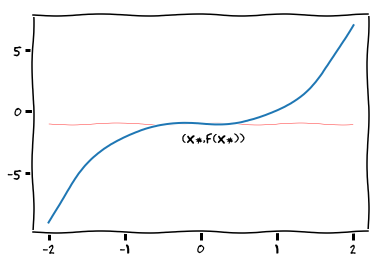
\includegraphics[width=0.5\linewidth]{x3.png}};
% % \draw [smooth, samples=100, domain=-1:1.442, blue, ultra thick, variable=\t] plot({\t}, {\t*\t*\t-1});
% % \draw[thick] (-2,-1) -- (2,-1);
% \draw[fill=blue] (0.1,0.125) circle (2pt); 
% % \draw (0.1,-0.2) node[scale=0.7] {$\big( \xstar, f(\xstar) \big)$};
% \end{tikzpicture}
% \end{tabular}
% \caption{On the left: the function is locally \emph{above} the tangent hyperplane at $\big(\xstar, f(\xstar)\big)$.  We have a local minimum at that location.  On the right, the graph crosses the tangent hyperplane.  We have no extrema at that location.}
% \label{figure:extrema}
% \end{figure}

% The following three results aid in our search for local extrema for twice-differentiable real-valued functions of one variable.

\begin{theorem}[Rolle's Theorem]\label{theorem:Rolle}
If $f\colon [a,b] \to \field{R}$ is a continuous function on a closed interval $[a,b]$, differentiable on $(a,b)$, and $f(a) = f(b)$, then there exists $c \in (a,b)$ so that $f'(c)=0$.
\end{theorem}

\begin{theorem}[Mean Value Theorem]\label{theorem:MVT}
If $f\colon [a,b] \to \field{R}$ is a continuous function on the closed interval $[a,b]$ and differentiable on $(a,b)$, then there exists $c \in (a,b)$ so that
\begin{equation*}
f'(c) = \frac{f(b)-f(a)}{b-a}
\end{equation*}
\end{theorem}

\begin{theorem}[Extended Law of the Mean]
If $f\colon D \to \field{R}$ is a twice differentiable function on a domain $D \subset \field{R}$ containing the closed interval $[a,b]$, then there exists $c \in (a,b)$ so that 
\begin{equation*}
f(b) = f(a) + f'(a)(b-a) + \tfrac{1}{2}f''(c)(b-a)^2
\end{equation*}
\end{theorem}

This last result can be extended to a real-valued function $f \colon \field{R}^ \to \field{R}$ as follows:

\begin{theorem}[Taylor]\label{theorem:Taylor}
Given two points $\boldsymbol{a}, \boldsymbol{b} \in \field{R}^d$, let $f\colon G \to \field{R}$ be a twice-differentiable real-valued function on an open set $G \subset \field{R}^d$ containing the segment $[\boldsymbol{a}, \boldsymbol{b}] = \{ \boldsymbol{a} + t (\boldsymbol{b} - \boldsymbol{a}) : t \in [0,1] \}$.  There exists $\boldsymbol{c} \in [\boldsymbol{a}, \boldsymbol{b}]$ so that 
\begin{equation*}
f(\x) = f(\boldsymbol{a}) + \langle \gradient{f}(\boldsymbol{a}), \x - \boldsymbol{a} \rangle + \frac{1}{2} \quadratic{\Hess{f}(c)} (\x-\boldsymbol{a})
\end{equation*}
\end{theorem}

% \begin{proof}
% Let's prove the first-dimensional case first:  Given $a,b \in \field{R}$, and a real-valued function $f\colon (a-\varepsilon, b+\varepsilon) \to \field{R}$ with continuous first and second derivatives in $(a-\varepsilon, b+\varepsilon)$ for some $\varepsilon>0$, we need to find the existence of a value $c \in [a,b]$ so that $f(x) = f(a) + f'(a)(x-a) + \tfrac{1}{2}f''(c)(x-a)^2$.

% Consider the Taylor polynomial of degree $n$ of $f$ at $x=a$, 
% \begin{equation*}
% T_n(x) = \sum_{k=0}^n \frac{f^{(k)}(a)}{k!}(x-a)^k
% \end{equation*}

% Consider the following piecewise functions $f_n(x)$:
% \begin{equation*}
% f_n(x) = \begin{cases} 
% \frac{f(x) - T_n(x)}{(x-a)^n} &\text{if }x\neq a \\
% 0 &\text{if }x=a
% \end{cases}
% \end{equation*}

% By using L'Hopital rule (up to two times where necessary), we can see that $\lim_{x \to a} f_n(x) = 0$. 

% Set $h(t) = f\big(\boldsymbol{a} + t (\boldsymbol{b} - \boldsymbol{a}) \big)$ to be the restriction of $f$ over the segment $[\boldsymbol{a},\boldsymbol{b}]$.  Note this function $h$ still has continuous first and second derivatives:
% \begin{align*}
% 	h'(t) = \gradient{f}
% \end{align*}
% \end{proof}

% TODO: We need to describe/prove Taylor's Formula (the extended Law of the
% Mean) and use it to figure out how to locate local minima

\begin{example}[Rosenbrock functions, continued]
In Example \ref{example:Rosenbrock2} we showed that the image of $\mathcal{R}_{a,b}$ is the interval $[0,\infty)$.  We also found (by inspection) that the point $(a,a^2)$ is a global minimum for this function. A straightforward computation shows that it is actually a strict global minimum.  A different approach to obtain this result can be obtained using the previous technique:
\begin{itemize}
	\item Notice $\mathcal{R}_{a,b}$ is twice differentiable.  Its gradient and Hessian are given respectively by
	\begin{equation*}
	\gradient{\mathcal{R}_{a,b}}(\x) = \big( 2(x_1-a) +4bx(x_1^2-x_2) , b(x_2-x_1^2) \big) \\
	\end{equation*}
	\begin{equation*}
	\Hess{\mathcal{R}_{a,b}}(\x) = \begin{bmatrix}
	12bx_1^2-4bx_2+2 & -4bx_1 \\
	-4bx_1 & 2b
	\end{bmatrix}
	\end{equation*}
	\item The search for critical points $\gradient{\mathcal{R}_{a,b}} = \boldsymbol{0}$ gives only the point $(a,a^2)$.
	\item The Hessian at that point is positive definite:
	\begin{equation*}
	\Hess{\mathcal{R}_{a,b}}(a,a^2) = \begin{bmatrix}
	8ba^2+2 & -4ab \\
	-4ab & 2b
	\end{bmatrix}
	\end{equation*}
\end{itemize}
\end{example}

\section{Optimization}


% TODO:  define the Rosenbrock function f(x,y)=(a-x)^2 + b(y-x^2)^2
%        compute its gradient, and use it to find critical points (there is only one: (a,a^2) )
%		 compute its Hessian, and prove that at (a,a^2), it is positive definite
%		 Use this to conclude that f has a global minimum at (a,a^2)
% Maybe extend this to higher dimensions?

\section*{Notes}
	